
\documentclass{article}
\usepackage{utf8math,ttquot,mathpartir,amsmath, amssymb, hydrocomments, mathtools,multicol,xspace}
\usepackage[margin=1in]{geometry}
\begin{document}

\abstract{Adding properties to hydroflow is important, because it
  allows us to do three things: (1) it lets us explicitly state and
  verify the requirements individual hydroflow operators have assumed
  of their inputs in order to be correct, (2) It allows us to encode
  translational goals and optimization correctness conditions, and (3) }

\section{technical todo}

\begin{itemize}
\item Type system: basic structure and derivations ✓
\item Type system: properties and their satisfaction
\item semantics: core semantic model (is it rewrite-based?)
\item Type system: axiom rewrite system
\item core language: axiom extensibility
\item proof: progress+preservation (or its equivalent in axiomatic semantics)
\item proof: axiom admissibility (via bisimulation?)
\item evaluation: example programs which satisfy the above
\item evaluation: programmability assessment
\item evaluation: extensibility assessment (new operators)
\end{itemize}

\section{syntax}

\newcommand{\closedprogram}{\textit{closed-program}\xspace}
\newcommand{\compiledcomponent}{\textit{compiled-component}\xspace}
\newcommand{\incast}{\textit{incast}\xspace}
\newcommand{\outcast}{\textit{outcast}\xspace}
\newcommand{\seqstart}{\textit{seq-start}\xspace}
\newcommand{\seqend}{\textit{seq-end}\xspace}
\newcommand{\chain}{\textit{chain}\xspace}
\newcommand{\op}{\textit{op}\xspace}
\newcommand{\opt}{τ_{\textit{op}}\xspace}
\newcommand{\N}{ℕ}
\newcommand{\fresh}{\textit{fresh}\xspace}
\newcommand{\inputs}{\textit{inputs}\xspace}
\newcommand{\outputs}{\textit{outputs}\xspace}
\newcommand{\IT}[1]{{\textit{#1}}\xspace}

\begin{figure}
  \begin{align*}
    \closedprogram &:= "declare"~ A…~"in"~ p\\
    A &∈ \textit{handoff-names}\\
    p_\IT{out} &:= [p_\IT{out}]\op ∣ A ∣ (p_\IT{out}|p_\IT{out})\\
    p_\IT{in} &:= [p_\IT{in}]\op ∣ A ∣ (p_\IT{in}|p_\IT{in})\\
    p &:= [p_\IT{in}]\op[p_\IT{out}] ∣ (p|p)
  \end{align*}
  \label{fig:syntax}
  \caption{Syntax}
\end{figure}


In figure \ref{fig:syntax}

\section{types}

\begin{figure}
  \begin{mathpar}

    {\inferrule{A : in(dₐ), A : out(dₐ),… ;A : τₐ,…;.  ⊢ p : τ}
      {⊢ "declare"~A…~"in"~p : τ}}
    
    {
      \inferrule{\inputs(\op) = τ \\ 
        C;Γ;. ⊢ p : τ \\ C';Γ';d.p.\op[0] ⊢ p' : τ'}
                {{C,C'};Γ,Γ';{d} ⊢ [p]\op[p'] : τ'}}
    
    {\inferrule[relevant-parallel]
      {C₁;Γ_1;d[n] ⊢ p₁ : τ₁ \\ C₂;Γ_2;d[n+1] ⊢ p₂ : τ₂}
      {C₁,C₂;Γ_1,Γ_2;d[n] ⊢ (p₁ ∣ p₂) : (τ₁ ∣ τ₂)}}

    {\inferrule[general-parallel]
      {C₁;Γ_1;. ⊢ p₁ : τ₁ \\ C₂;Γ_2;. ⊢ p₂ : τ₂}
      {C₁,C₂;Γ_1,Γ_2; . ⊢ (p₁ ∣ p₂) : (τ₁ ∣ τ₂)}}

    {\inferrule[exchange-C]
      {C,C_2,C_1,C' ;Γ; d ⊢ p : τ}
      {C,C_1,C_2,C' ;Γ; d ⊢ p : τ}}

    {\inferrule[exchange-gamma]
      {C ;Γ,Γ_1,Γ_2,Γ' ; d ⊢ p : τ}
      {C ;Γ,Γ_2,Γ_1,Γ'; d ⊢ p : τ}}

    {\inferrule[weaken-gamma]
      {C ;Γ,Γ' ; d ⊢ p : τ}
      {C ;Γ,Γ_w,Γ'; d ⊢ p : τ}}

    {\inferrule[contract-gamma]
      {C ;Γ,Γ_c,Γ_c,Γ' ; d ⊢ p : τ}
      {C ;Γ,Γ_c,Γ'; d ⊢ p : τ}}


    {\inferrule[unfold]{A:d',C;Γ;d[A/d] ⊢ p : τ}{A:d',C;Γ;d ⊢ p : τ}}

    {\inferrule[fold]{A:d',C;Γ;d⊢ p : τ}{A:d',C;Γ;d[A/d]⊢ p : τ}}

    {\inferrule[varref-out]{Γ ⊢ d : τ}{A:out(d);Γ;d ⊢ A : τ}}

    {\inferrule[varref-in]{}{A:in(d);A : τ; . ⊢ A : τ}}
      
    \end{mathpar}\MPM{There's something fishy going on with varref-in; right now, you could use it and then immediately apply unfold to get a derivation which might not typecheck. We need to prove this is not actually a problem.}
    %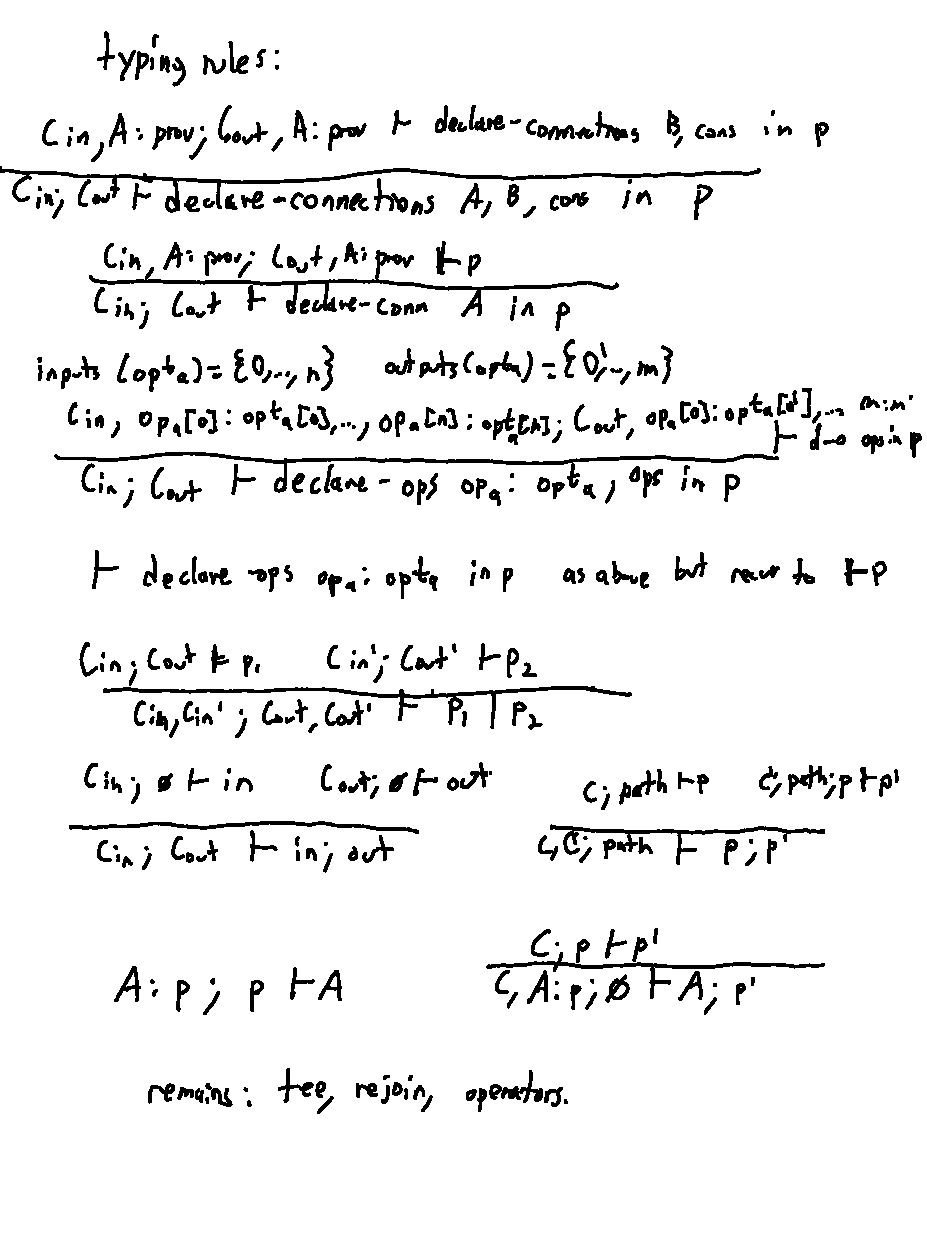
\includegraphics{freehand-types}
  \label{fig:types}
  \caption{Types}
\end{figure}

We're not bothering with the oaklandish split right now, it's too
silly.  Open question if we need the relevance version of the rule, or
can remove the $:^r$ annotation and observe that the $[n]$ version is
only ever used with empty contexts for inputs to operators. Also worth
wondering if we're going to be in trouble overloading the [] syntax
here; time will tell. Types appear in figure \ref{fig:types}

\section{general notes}

Something we originally wanted to do was relaxations---operators that happened to consume input $'s$, but could just as well accept any $"permute"('s)$.  How do we want to model this relaxation now, and is it still in scope? Concretely, I believe that this _is_ still in scope, and takes the form of setting translation-preservation targets to literal expressions like $"permute"('s)$.  The challenge here will be reasoning in the algebra; we're not talking about equational rewriting anymore, since we also need to include weakening ("permute" generalizes lots of transformations). 


\end{document}
